% ==============================================================================
% Section 3: Empirical Data Ingestion & Return Diagnostics
% ==============================================================================

\section{Data Collection and Return Diagnostics}
\label{sec:return_diagnostics}

Daily historical adjusted closing prices for ITC Limited were ingested from the National Stock Exchange of India (NSE: \texttt{ITC.NS}) over a trailing 1-year window from \textbf{17 November 2025 to 16 November 2026}. The sample comprises $N = 246$ consecutive daily return observations. Daily continuously compounded log returns are computed as:
\begin{equation}
R_t = \ln\left(\frac{P_t}{P_{t-1}}\right) = \ln(P_t) - \ln(P_{t-1})
\label{eq:log_return}
\end{equation}

Table~\ref{tab:descriptive_stats} presents the summary statistics alongside annualized metrics based on the standard 252-day Indian financial market convention.

\begin{table}[htbp]
\centering
\small
\caption{Descriptive Statistics for Daily Log Returns of ITC Limited ($N = 246$)}
\label{tab:descriptive_stats}
\begin{tabularx}{0.92\linewidth}{lXrr}
\toprule
\textbf{Statistic Metric} & \textbf{Notation / Formula} & \textbf{Daily Value} & \textbf{Annualized Value} \\
\midrule
Sample Size ($N$) & Clean trading sessions & $246$ & -- \\
Sample Period & Historical window & 17-Nov-2025 to 16-Nov-2026 & 1.0 Year \\
Reference Spot Price & $S_0$ (NSE Close) & \rupee 285.00 & -- \\
Position Lot Exposure & $V_0 = 1,725 \times S_0$ & \rupee 4,91,625.00 & -- \\
Mean Log Return & $\hat{\mu} = \frac{1}{N}\sum R_t$ & $-0.001114$ & $-28.0811\%$ \\
Sample Volatility & $\hat{\sigma} = \sqrt{\frac{1}{N-1}\sum (R_t - \hat{\mu})^2}$ & $0.014742$ & $23.4019\%$ \\
Sample Skewness & $\hat{S} = \frac{1}{N}\sum (R_t - \hat{\mu})^3 / \hat{\sigma}^3$ & $-0.9243$ & -- \\
Excess Kurtosis & $\hat{K}_{\text{excess}} = \frac{1}{N}\sum (R_t - \hat{\mu})^4 / \hat{\sigma}^4 - 3$ & $+9.8233$ & Raw: $12.8233$ \\
Jarque--Bera Statistic & $JB = \frac{N}{6}\left(S^2 + \frac{K_{\text{excess}}^2}{4}\right)$ & $979.34$ & $p = 2.18 \times 10^{-213}$ \\
\bottomrule
\end{tabularx}
\end{table}

\subsection{Testing the Gaussian Normality Hypothesis}

Under the null hypothesis of Gaussian normality ($H_0: S = 0 \text{ and } K_{\text{excess}} = 0$), the Jarque--Bera ($JB$) statistic asymptotically follows a Chi-Square distribution with two degrees of freedom ($\chi^2(2)$). The finite-sample test yields $JB = 979.34$, with an associated $p$-value of $p = 2.18 \times 10^{-213}$. Because $979.34 \gg \chi^2_{0.05, 2} = 5.9915$, the hypothesis of Gaussian normality is decisively rejected.

\begin{figure}[htbp]
\centering
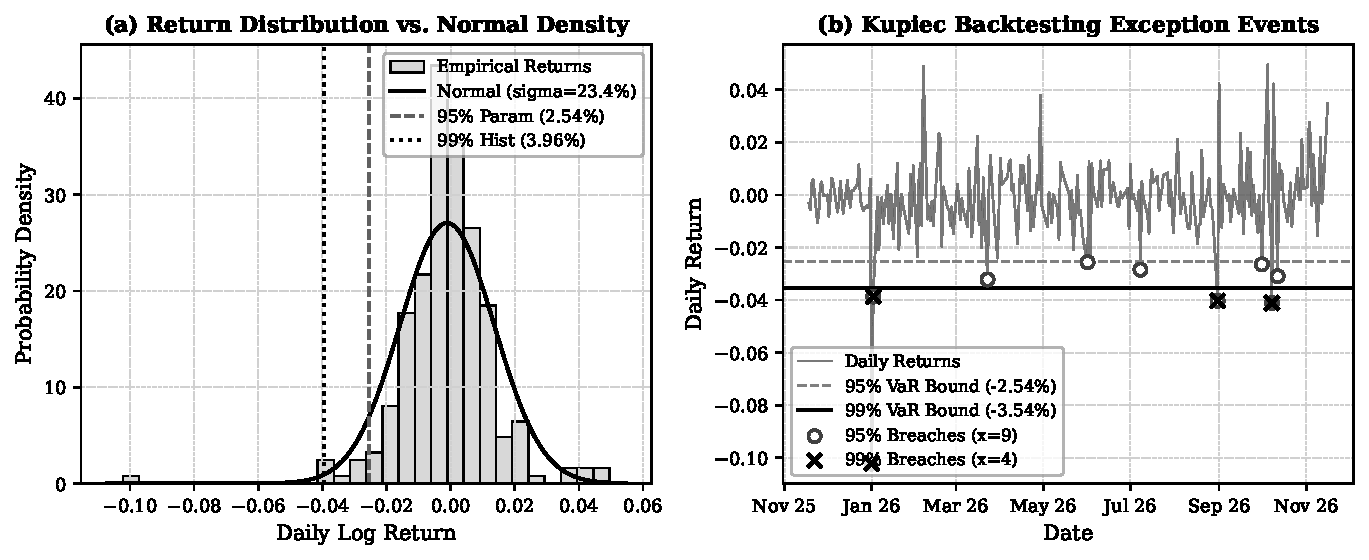
\includegraphics[width=0.98\linewidth]{figures/fig1_diagnostics_backtest.pdf}
\caption{Empirical Return Diagnostics and Kupiec Backtesting Exception Events}
\label{fig:diagnostics_backtest}
\vspace{2pt}
\begin{minipage}{0.96\linewidth}
\footnotesize\textbf{Note:} (a) Empirical daily log return distribution vs. fitted normal density ($\sigma_{\text{ann}} = 23.40\%$) showing $95\%$ and $99\%$ $\VaR$ cutoffs. (b) Kupiec backtesting timeline showing daily returns and tail violation events ($x = 9$ breaches at $95\%$; $x = 4$ breaches at $99\%$).
\end{minipage}
\end{figure}

As visually documented in Figure~\ref{fig:diagnostics_backtest}(a), the empirical distribution is characterized by severe central peakedness and an extended negative crash tail. This confirms that classical parametric models assuming Gaussian bell curves will systematically underpredict tail loss severity during adverse market conditions.
